\documentclass[12pt,a4paper]{article}

\usepackage[a4paper,text={16.5cm,25.2cm},centering]{geometry}
\usepackage{lmodern}
\usepackage{amssymb,amsmath}
\usepackage{bm}
\usepackage{graphicx}
\usepackage{microtype}
\usepackage{hyperref}
\usepackage{mhchem}
\setlength{\parindent}{0pt}
\setlength{\parskip}{1.2ex}

\hypersetup
       {   pdfauthor = {  },
           pdftitle={  },
           colorlinks=TRUE,
           linkcolor=black,
           citecolor=blue,
           urlcolor=blue
       }




\usepackage{upquote}
\usepackage{listings}
\usepackage{xcolor}
\lstset{
    basicstyle=\ttfamily\footnotesize,
    upquote=true,
    breaklines=true,
    breakindent=0pt,
    keepspaces=true,
    showspaces=false,
    columns=fullflexible,
    showtabs=false,
    showstringspaces=false,
    escapeinside={(*@}{@*)},
    extendedchars=true,
}
\newcommand{\HLJLt}[1]{#1}
\newcommand{\HLJLw}[1]{#1}
\newcommand{\HLJLe}[1]{#1}
\newcommand{\HLJLeB}[1]{#1}
\newcommand{\HLJLo}[1]{#1}
\newcommand{\HLJLk}[1]{\textcolor[RGB]{148,91,176}{\textbf{#1}}}
\newcommand{\HLJLkc}[1]{\textcolor[RGB]{59,151,46}{\textit{#1}}}
\newcommand{\HLJLkd}[1]{\textcolor[RGB]{214,102,97}{\textit{#1}}}
\newcommand{\HLJLkn}[1]{\textcolor[RGB]{148,91,176}{\textbf{#1}}}
\newcommand{\HLJLkp}[1]{\textcolor[RGB]{148,91,176}{\textbf{#1}}}
\newcommand{\HLJLkr}[1]{\textcolor[RGB]{148,91,176}{\textbf{#1}}}
\newcommand{\HLJLkt}[1]{\textcolor[RGB]{148,91,176}{\textbf{#1}}}
\newcommand{\HLJLn}[1]{#1}
\newcommand{\HLJLna}[1]{#1}
\newcommand{\HLJLnb}[1]{#1}
\newcommand{\HLJLnbp}[1]{#1}
\newcommand{\HLJLnc}[1]{#1}
\newcommand{\HLJLncB}[1]{#1}
\newcommand{\HLJLnd}[1]{\textcolor[RGB]{214,102,97}{#1}}
\newcommand{\HLJLne}[1]{#1}
\newcommand{\HLJLneB}[1]{#1}
\newcommand{\HLJLnf}[1]{\textcolor[RGB]{66,102,213}{#1}}
\newcommand{\HLJLnfm}[1]{\textcolor[RGB]{66,102,213}{#1}}
\newcommand{\HLJLnp}[1]{#1}
\newcommand{\HLJLnl}[1]{#1}
\newcommand{\HLJLnn}[1]{#1}
\newcommand{\HLJLno}[1]{#1}
\newcommand{\HLJLnt}[1]{#1}
\newcommand{\HLJLnv}[1]{#1}
\newcommand{\HLJLnvc}[1]{#1}
\newcommand{\HLJLnvg}[1]{#1}
\newcommand{\HLJLnvi}[1]{#1}
\newcommand{\HLJLnvm}[1]{#1}
\newcommand{\HLJLl}[1]{#1}
\newcommand{\HLJLld}[1]{\textcolor[RGB]{148,91,176}{\textit{#1}}}
\newcommand{\HLJLs}[1]{\textcolor[RGB]{201,61,57}{#1}}
\newcommand{\HLJLsa}[1]{\textcolor[RGB]{201,61,57}{#1}}
\newcommand{\HLJLsb}[1]{\textcolor[RGB]{201,61,57}{#1}}
\newcommand{\HLJLsc}[1]{\textcolor[RGB]{201,61,57}{#1}}
\newcommand{\HLJLsd}[1]{\textcolor[RGB]{201,61,57}{#1}}
\newcommand{\HLJLsdB}[1]{\textcolor[RGB]{201,61,57}{#1}}
\newcommand{\HLJLsdC}[1]{\textcolor[RGB]{201,61,57}{#1}}
\newcommand{\HLJLse}[1]{\textcolor[RGB]{59,151,46}{#1}}
\newcommand{\HLJLsh}[1]{\textcolor[RGB]{201,61,57}{#1}}
\newcommand{\HLJLsi}[1]{#1}
\newcommand{\HLJLso}[1]{\textcolor[RGB]{201,61,57}{#1}}
\newcommand{\HLJLsr}[1]{\textcolor[RGB]{201,61,57}{#1}}
\newcommand{\HLJLss}[1]{\textcolor[RGB]{201,61,57}{#1}}
\newcommand{\HLJLssB}[1]{\textcolor[RGB]{201,61,57}{#1}}
\newcommand{\HLJLnB}[1]{\textcolor[RGB]{59,151,46}{#1}}
\newcommand{\HLJLnbB}[1]{\textcolor[RGB]{59,151,46}{#1}}
\newcommand{\HLJLnfB}[1]{\textcolor[RGB]{59,151,46}{#1}}
\newcommand{\HLJLnh}[1]{\textcolor[RGB]{59,151,46}{#1}}
\newcommand{\HLJLni}[1]{\textcolor[RGB]{59,151,46}{#1}}
\newcommand{\HLJLnil}[1]{\textcolor[RGB]{59,151,46}{#1}}
\newcommand{\HLJLnoB}[1]{\textcolor[RGB]{59,151,46}{#1}}
\newcommand{\HLJLoB}[1]{\textcolor[RGB]{102,102,102}{\textbf{#1}}}
\newcommand{\HLJLow}[1]{\textcolor[RGB]{102,102,102}{\textbf{#1}}}
\newcommand{\HLJLp}[1]{#1}
\newcommand{\HLJLc}[1]{\textcolor[RGB]{153,153,119}{\textit{#1}}}
\newcommand{\HLJLch}[1]{\textcolor[RGB]{153,153,119}{\textit{#1}}}
\newcommand{\HLJLcm}[1]{\textcolor[RGB]{153,153,119}{\textit{#1}}}
\newcommand{\HLJLcp}[1]{\textcolor[RGB]{153,153,119}{\textit{#1}}}
\newcommand{\HLJLcpB}[1]{\textcolor[RGB]{153,153,119}{\textit{#1}}}
\newcommand{\HLJLcs}[1]{\textcolor[RGB]{153,153,119}{\textit{#1}}}
\newcommand{\HLJLcsB}[1]{\textcolor[RGB]{153,153,119}{\textit{#1}}}
\newcommand{\HLJLg}[1]{#1}
\newcommand{\HLJLgd}[1]{#1}
\newcommand{\HLJLge}[1]{#1}
\newcommand{\HLJLgeB}[1]{#1}
\newcommand{\HLJLgh}[1]{#1}
\newcommand{\HLJLgi}[1]{#1}
\newcommand{\HLJLgo}[1]{#1}
\newcommand{\HLJLgp}[1]{#1}
\newcommand{\HLJLgs}[1]{#1}
\newcommand{\HLJLgsB}[1]{#1}
\newcommand{\HLJLgt}[1]{#1}


\begin{document}



\section{Introduction to GPU Programming}
The following tutorials assume that you have have setup \href{https://github.com/JuliaGPU/CUDA.jl}{CUDA.jl}. Detailed installation instructions can be found \href{https://juliagpu.gitlab.io/CUDA.jl/installation/overview/#InstallationOverview}{here}.

You may check if your \texttt{CUDA.jl} installation is functional using 


\begin{lstlisting}
(*@\HLJLk{using}@*) (*@\HLJLn{CUDA}@*)
(*@\HLJLn{CUDA}@*)(*@\HLJLoB{.}@*)(*@\HLJLnf{functional}@*)(*@\HLJLp{()}@*)
\end{lstlisting}

\begin{lstlisting}
true
\end{lstlisting}


If \texttt{CUDA.functional()} returns false then the package is in a non-functional state and you should follow the \href{https://juliagpu.gitlab.io/CUDA.jl/installation/overview/}{documentation} to get it working.

Also explained in the \href{https://juliagpu.gitlab.io/CUDA.jl/usage/overview/}{usage} section of the \texttt{CUDA.jl} \href{https://juliagpu.gitlab.io/CUDA.jl/}{docs} is an overview of \texttt{CUDA.jl}'s functionality which can work at three distinct levels.

\begin{itemize}
\item Array Abstractions: With the help of the \texttt{CuArray} type we can use Base's array abstractions like broadcasting and mapreduce. 


\item Native Kernels: Write kernels which compiles to native GPU code directly from Julia.


\item CUDA API wrappers: Call CUDA libraries directly from Julia for bleeding edge performance.

\end{itemize}
The purpose of these tutorials is to teach you effective GPU programming. The tutorials here complement other GPU programming resources such as the NVIDIA blogs, other online resources and formal textbooks. Using other resources in your study will complement these tutorials and is highly encouraged.

A GPU (graphical processing unit) is a device specially designed for graphics work. Graphical tasks are a good candidate for parallelization and  GPU's exploit it by having a large number of less powerful processors instead of a single very powerful processor. In 2007 NVIDIA released CUDA (Compute Unified Device Architecture), a parallel programming platform (hardware and software stack) which alongside graphics also focusses scientific computation. Modern GPU's are commonly called GPGPU (general purpose GPU) which shows their importance in scientific computation alongside graphics.

Programs which execute on the GPU are vastly different due to its different architecture. There are new paradigms and algorithms to learn. Understanding how a GPU works is crucial to maximizing the performance of your application.

\section{Parallelizing AXPY}
\href{https://en.wikipedia.org/wiki/Basic_Linear_Algebra_Subprograms}{Basic Linear Algebra Subroutines(BLAS)} are subroutines for Linear Algebra operations. Linear algebra's importance in scientific computing makes BLAS essential to GPU computing. One of the most primitive BLAS operations is to add a scaled vector to another vector. Given two vectors ($x$ and $y$) and a scalar ($\alpha$) we add $\alpha\cdot x$ to $y$. In BLAS libraries this manifests as the functions SAXPY, DAXPY and CAXPY. The difference between the three is that the data type of the vectors is \texttt{Float32}, \texttt{Float64} and \texttt{Complex\{Float32\}} respectively. However in this example we call our subroutine \texttt{axpy} and let Julia take care of the types.


\begin{lstlisting}
(*@\HLJLk{function}@*) (*@\HLJLnf{axpy!}@*)(*@\HLJLp{(}@*)(*@\HLJLn{A}@*)(*@\HLJLp{,}@*) (*@\HLJLn{X}@*)(*@\HLJLp{,}@*) (*@\HLJLn{Y}@*)(*@\HLJLp{)}@*) 
    (*@\HLJLk{for}@*) (*@\HLJLn{i}@*) (*@\HLJLkp{in}@*) (*@\HLJLnf{eachindex}@*)(*@\HLJLp{(}@*)(*@\HLJLn{Y}@*)(*@\HLJLp{)}@*)
        (*@\HLJLnd{@inbounds}@*) (*@\HLJLn{Y}@*)(*@\HLJLp{[}@*)(*@\HLJLn{i}@*)(*@\HLJLp{]}@*) (*@\HLJLoB{=}@*) (*@\HLJLn{A}@*) (*@\HLJLoB{*}@*) (*@\HLJLn{X}@*)(*@\HLJLp{[}@*)(*@\HLJLn{i}@*)(*@\HLJLp{]}@*) (*@\HLJLoB{+}@*) (*@\HLJLn{Y}@*)(*@\HLJLp{[}@*)(*@\HLJLn{i}@*)(*@\HLJLp{]}@*)
    (*@\HLJLk{end}@*)
(*@\HLJLk{end}@*)

(*@\HLJLn{N}@*) (*@\HLJLoB{=}@*) (*@\HLJLni{2}@*)(*@\HLJLoB{{\textasciicircum}}@*)(*@\HLJLni{29}@*)
(*@\HLJLn{v1}@*) (*@\HLJLoB{=}@*) (*@\HLJLnf{rand}@*)(*@\HLJLp{(}@*)(*@\HLJLn{Float32}@*)(*@\HLJLp{,}@*) (*@\HLJLn{N}@*)(*@\HLJLp{)}@*)
(*@\HLJLn{v2}@*) (*@\HLJLoB{=}@*) (*@\HLJLnf{rand}@*)(*@\HLJLp{(}@*)(*@\HLJLn{Float32}@*)(*@\HLJLp{,}@*) (*@\HLJLn{N}@*)(*@\HLJLp{)}@*)
(*@\HLJLn{v2{\_}copy}@*) (*@\HLJLoB{=}@*) (*@\HLJLnf{copy}@*)(*@\HLJLp{(}@*)(*@\HLJLn{v2}@*)(*@\HLJLp{)}@*) (*@\HLJLcs{{\#}}@*) (*@\HLJLcs{maintain}@*) (*@\HLJLcs{a}@*) (*@\HLJLcs{copy}@*) (*@\HLJLcs{of}@*) (*@\HLJLcs{the}@*) (*@\HLJLcs{original}@*)
(*@\HLJLn{\ensuremath{\alpha}}@*) (*@\HLJLoB{=}@*) (*@\HLJLnf{rand}@*)(*@\HLJLp{()}@*)

(*@\HLJLnf{axpy!}@*)(*@\HLJLp{(}@*)(*@\HLJLn{\ensuremath{\alpha}}@*)(*@\HLJLp{,}@*) (*@\HLJLn{v1}@*)(*@\HLJLp{,}@*) (*@\HLJLn{v2}@*)(*@\HLJLp{)}@*)
\end{lstlisting}


Alternatively, we can also use Julia's \href{https://docs.julialang.org/en/v1/manual/arrays/#Broadcasting}{broadcasting} syntax which allows us to write it in simpler and equally performant version. 

v3 = copy(v2\_copy) v3 .+= \ensuremath{\alpha} * v1

@show v2 == v3

\subsubsection{CPU multithreaded version}
Consider parallelization with \texttt{p} processors. We can divide our arrays into \texttt{p} subarrays of equal size and assign a processor to each subarray. This can theoretically make our parallel version \texttt{p} times faster. We say "theoretically" because there is an overhead of starting threads and synchronizing them. Our hope in parallel computing is that the cost will get amortized with the speedup of parallelization but that may not be the case. Which is why measuring performance is extremely important. Nevertheless, the parallel version scales linearly w.r.t \texttt{p} which is really good, so much so that these types of problems are classified as "embarassingly parallel". In other cases when processors need to communicate and synchronize frquently the benefit does not scale linearly with the number of processors.

We can use Julia's inbuilt multithreading functionality to use multiple CPU threads which is documented(\href{https://docs.julialang.org/en/v1/manual/multi-threading/}{here}). You need to ensure that Julia starts with the appropriate number of threads using the environment variable or startup option(\texttt{-t NUMTHREADS}), instructions for which are given in the docs.

A common theme in parallel computing is the concept of thread rank or id. Each thread has a unique id/rank which helps us identify them and map them to tasks easily.


\begin{lstlisting}
(*@\HLJLk{using}@*) (*@\HLJLn{Base}@*)(*@\HLJLoB{.}@*)(*@\HLJLn{Threads}@*)

(*@\HLJLnf{println}@*)(*@\HLJLp{(}@*)(*@\HLJLs{"{}Number}@*) (*@\HLJLs{of}@*) (*@\HLJLs{CPU}@*) (*@\HLJLs{threads}@*) (*@\HLJLs{=}@*) (*@\HLJLs{"{}}@*)(*@\HLJLp{,}@*) (*@\HLJLnf{nthreads}@*)(*@\HLJLp{())}@*)

(*@\HLJLcs{{\#}}@*) (*@\HLJLcs{pseudocode}@*) (*@\HLJLcs{for}@*) (*@\HLJLcs{parallel}@*) (*@\HLJLcs{saxpy}@*)
(*@\HLJLk{function}@*) (*@\HLJLnf{parallel{\_}axpy!}@*)(*@\HLJLp{(}@*)(*@\HLJLn{A}@*)(*@\HLJLp{,}@*) (*@\HLJLn{X}@*)(*@\HLJLp{,}@*) (*@\HLJLn{Y}@*)(*@\HLJLp{)}@*)
    (*@\HLJLn{len}@*) (*@\HLJLoB{=}@*) (*@\HLJLnf{cld}@*)(*@\HLJLp{(}@*)(*@\HLJLnf{length}@*)(*@\HLJLp{(}@*)(*@\HLJLn{X}@*)(*@\HLJLp{),}@*) (*@\HLJLnf{nthreads}@*)(*@\HLJLp{())}@*)

    (*@\HLJLcs{{\#}}@*) (*@\HLJLcs{Launch}@*) (*@\HLJLcs{threads}@*) (*@\HLJLcs{=}@*) (*@\HLJLcs{nthreads()}@*)
    (*@\HLJLn{Threads}@*)(*@\HLJLoB{.}@*)(*@\HLJLnd{@threads}@*) (*@\HLJLk{for}@*) (*@\HLJLn{i}@*) (*@\HLJLkp{in}@*) (*@\HLJLni{1}@*)(*@\HLJLoB{:}@*)(*@\HLJLnf{nthreads}@*)(*@\HLJLp{()}@*)
        (*@\HLJLcs{{\#}}@*) (*@\HLJLcs{set}@*) (*@\HLJLcs{id}@*) (*@\HLJLcs{to}@*) (*@\HLJLcs{thread}@*) (*@\HLJLcs{rank/id}@*)
        (*@\HLJLn{tid}@*) (*@\HLJLoB{=}@*) (*@\HLJLnf{threadid}@*)(*@\HLJLp{()}@*)
        (*@\HLJLn{low}@*) (*@\HLJLoB{=}@*) (*@\HLJLni{1}@*) (*@\HLJLoB{+}@*) (*@\HLJLp{(}@*)(*@\HLJLn{tid}@*) (*@\HLJLoB{-}@*) (*@\HLJLni{1}@*)(*@\HLJLp{)}@*)(*@\HLJLoB{*}@*)(*@\HLJLn{len}@*)
        (*@\HLJLn{high}@*) (*@\HLJLoB{=}@*) (*@\HLJLnf{min}@*)(*@\HLJLp{(}@*)(*@\HLJLnf{length}@*)(*@\HLJLp{(}@*)(*@\HLJLn{X}@*)(*@\HLJLp{),}@*) (*@\HLJLn{len}@*) (*@\HLJLoB{*}@*) (*@\HLJLn{tid}@*)(*@\HLJLp{)}@*) (*@\HLJLcs{{\#}}@*) (*@\HLJLcs{The}@*) (*@\HLJLcs{last}@*) (*@\HLJLcs{segment}@*) (*@\HLJLcs{might}@*) (*@\HLJLcs{have}@*) (*@\HLJLcs{lesser}@*) (*@\HLJLcs{elements}@*) (*@\HLJLcs{than}@*) (*@\HLJLcs{len}@*)

        (*@\HLJLcs{{\#}}@*) (*@\HLJLcs{Broadcast}@*) (*@\HLJLcs{syntax,}@*) (*@\HLJLcs{views}@*) (*@\HLJLcs{used}@*) (*@\HLJLcs{to}@*) (*@\HLJLcs{avoid}@*) (*@\HLJLcs{copying}@*)
        (*@\HLJLnf{view}@*)(*@\HLJLp{(}@*)(*@\HLJLn{Y}@*)(*@\HLJLp{,}@*) (*@\HLJLn{low}@*)(*@\HLJLoB{:}@*)(*@\HLJLn{high}@*)(*@\HLJLp{)}@*) (*@\HLJLoB{.+=}@*) (*@\HLJLn{A}@*)(*@\HLJLoB{.*}@*)(*@\HLJLnf{view}@*)(*@\HLJLp{(}@*)(*@\HLJLn{X}@*)(*@\HLJLp{,}@*) (*@\HLJLn{low}@*)(*@\HLJLoB{:}@*)(*@\HLJLn{high}@*)(*@\HLJLp{)}@*)
    (*@\HLJLk{end}@*)
    (*@\HLJLk{return}@*)
(*@\HLJLk{end}@*)

(*@\HLJLn{v4}@*) (*@\HLJLoB{=}@*) (*@\HLJLnf{copy}@*)(*@\HLJLp{(}@*)(*@\HLJLn{v2{\_}copy}@*)(*@\HLJLp{)}@*)
(*@\HLJLnf{parallel{\_}axpy!}@*)(*@\HLJLp{(}@*)(*@\HLJLn{\ensuremath{\alpha}}@*)(*@\HLJLp{,}@*) (*@\HLJLn{v1}@*)(*@\HLJLp{,}@*) (*@\HLJLn{v4}@*)(*@\HLJLp{)}@*)

(*@\HLJLnd{@show}@*) (*@\HLJLn{v2}@*) (*@\HLJLoB{==}@*) (*@\HLJLn{v4}@*)
\end{lstlisting}

\begin{lstlisting}
Number of CPU threads = 6
v2 == v4 = true
true
\end{lstlisting}


\subsubsection{GPU version}
Given below is the code for GPU


\begin{lstlisting}
(*@\HLJLk{function}@*) (*@\HLJLnf{gpu{\_}axpy!}@*)(*@\HLJLp{(}@*)(*@\HLJLn{A}@*)(*@\HLJLp{,}@*) (*@\HLJLn{X}@*)(*@\HLJLp{,}@*) (*@\HLJLn{Y}@*)(*@\HLJLp{)}@*) 
    (*@\HLJLcs{{\#}}@*) (*@\HLJLcs{set}@*) (*@\HLJLcs{tid}@*) (*@\HLJLcs{to}@*) (*@\HLJLcs{thread}@*) (*@\HLJLcs{rank}@*)
    (*@\HLJLn{tid}@*) (*@\HLJLoB{=}@*) (*@\HLJLp{(}@*)(*@\HLJLnf{blockIdx}@*)(*@\HLJLp{()}@*)(*@\HLJLoB{.}@*)(*@\HLJLn{x}@*) (*@\HLJLoB{-}@*) (*@\HLJLni{1}@*)(*@\HLJLp{)}@*) (*@\HLJLoB{*}@*) (*@\HLJLnf{blockDim}@*)(*@\HLJLp{()}@*)(*@\HLJLoB{.}@*)(*@\HLJLn{x}@*) (*@\HLJLoB{+}@*) (*@\HLJLnf{threadIdx}@*)(*@\HLJLp{()}@*)(*@\HLJLoB{.}@*)(*@\HLJLn{x}@*)
    (*@\HLJLn{tid}@*) (*@\HLJLoB{>}@*) (*@\HLJLnf{length}@*)(*@\HLJLp{(}@*)(*@\HLJLn{Y}@*)(*@\HLJLp{)}@*) (*@\HLJLoB{{\&}{\&}}@*) (*@\HLJLk{return}@*) 
    (*@\HLJLnd{@inbounds}@*) (*@\HLJLn{Y}@*)(*@\HLJLp{[}@*)(*@\HLJLn{tid}@*)(*@\HLJLp{]}@*) (*@\HLJLoB{=}@*) (*@\HLJLn{A}@*)(*@\HLJLoB{*}@*)(*@\HLJLn{X}@*)(*@\HLJLp{[}@*)(*@\HLJLn{tid}@*)(*@\HLJLp{]}@*) (*@\HLJLoB{+}@*) (*@\HLJLn{Y}@*)(*@\HLJLp{[}@*)(*@\HLJLn{tid}@*)(*@\HLJLp{]}@*)
    (*@\HLJLk{return}@*)
(*@\HLJLk{end}@*)

(*@\HLJLcs{{\#}}@*) (*@\HLJLcs{Transfer}@*) (*@\HLJLcs{array}@*) (*@\HLJLcs{to}@*) (*@\HLJLcs{GPU}@*) (*@\HLJLcs{memory}@*)
(*@\HLJLn{gpu{\_}v1}@*) (*@\HLJLoB{=}@*) (*@\HLJLnf{CuArray}@*)(*@\HLJLp{(}@*)(*@\HLJLn{v1}@*)(*@\HLJLp{)}@*)
(*@\HLJLn{gpu{\_}v2}@*) (*@\HLJLoB{=}@*) (*@\HLJLnf{CuArray}@*)(*@\HLJLp{(}@*)(*@\HLJLn{v2{\_}copy}@*)(*@\HLJLp{)}@*)

(*@\HLJLn{numthreads}@*) (*@\HLJLoB{=}@*) (*@\HLJLni{256}@*)
(*@\HLJLn{numblocks}@*) (*@\HLJLoB{=}@*) (*@\HLJLnf{cld}@*)(*@\HLJLp{(}@*)(*@\HLJLn{N}@*)(*@\HLJLp{,}@*) (*@\HLJLn{numthreads}@*)(*@\HLJLp{)}@*)

(*@\HLJLnd{@show}@*) (*@\HLJLn{numthreads}@*)
(*@\HLJLnd{@show}@*) (*@\HLJLn{numblocks}@*)

(*@\HLJLcs{{\#}}@*) (*@\HLJLcs{Launch}@*) (*@\HLJLcs{the}@*) (*@\HLJLcs{gpu{\_}axpy!}@*) (*@\HLJLcs{on}@*) (*@\HLJLcs{the}@*) (*@\HLJLcs{GPU}@*)
(*@\HLJLnd{@cuda}@*) (*@\HLJLn{threads}@*)(*@\HLJLoB{=}@*)(*@\HLJLn{numthreads}@*) (*@\HLJLn{blocks}@*)(*@\HLJLoB{=}@*)(*@\HLJLn{numblocks}@*) (*@\HLJLnf{gpu{\_}axpy!}@*)(*@\HLJLp{(}@*)(*@\HLJLn{\ensuremath{\alpha}}@*)(*@\HLJLp{,}@*) (*@\HLJLn{gpu{\_}v1}@*)(*@\HLJLp{,}@*) (*@\HLJLn{gpu{\_}v2}@*)(*@\HLJLp{)}@*)

(*@\HLJLcs{{\#}}@*) (*@\HLJLcs{Copy}@*) (*@\HLJLcs{back}@*) (*@\HLJLcs{to}@*) (*@\HLJLcs{RAM}@*)
(*@\HLJLn{v4}@*) (*@\HLJLoB{=}@*) (*@\HLJLnf{Array}@*)(*@\HLJLp{(}@*)(*@\HLJLn{gpu{\_}v2}@*)(*@\HLJLp{)}@*)

(*@\HLJLcs{{\#}}@*) (*@\HLJLcs{Verify}@*) (*@\HLJLcs{that}@*) (*@\HLJLcs{the}@*) (*@\HLJLcs{answers}@*) (*@\HLJLcs{are}@*) (*@\HLJLcs{the}@*) (*@\HLJLcs{same}@*)
(*@\HLJLnd{@show}@*) (*@\HLJLn{v2}@*) (*@\HLJLoB{==}@*) (*@\HLJLn{v4}@*)
\end{lstlisting}

\begin{lstlisting}
numthreads = 256
numblocks = 2097152
v2 == v4 = true
true
\end{lstlisting}


Compared to the CPU code there are a number of differences which need to be addressed.

\subparagraph{1) Thread Indexing}
The multithreaded CPU code used \texttt{threadid()} to get the current thread's rank whereas on the GPU the complicated expression \texttt{tid = (blockIdx().x - 1) * blockDim().x + threadIdx().x} computed rank. Furthermore, we are using two distinct terms, \texttt{blocks} and \texttt{threads}.

\subparagraph{2) SIMT architecture}
The multithreaded CPU code divided the array up into a handful of pieces equal to the number of processors. A modern CPU has a handful of cores(4 - 8), hence each thread still works on a relatively large array whereas the GPU processes one element per thread. While both demonstrate parallelism their scales differ vastly.

Flynn's taxonomy is a popular way to classify parallel computer architectures.

\begin{tabular}
{l | l | l}
x & single data & multiple data \\
\hline
single instruction & SISD & SIMD \\
multiple instruction & MISD & MIMD \\
\end{tabular}
\begin{itemize}
\item SISD(single instruction single data) is the classical uniprocessor model. A single instruction stream executes and acts on a single data element at a time.


\item SIMD(single instruction multiple data) incorporates a level of parallelism by having a single instruction stream acting on multiple data elements at a time. An example of this is vectorized CPU instructions which use large registers containing multiple data elements. Instructions that work with these large vector registers effectively work on multiple data elements in parallel with a single instruction utilizing special hardware.


\item MISD (multiple instruction single data) is currently only a theoretical model and no commercial machine has been built which uses it.


\item MIMD (multiple instruction multiple data) is able to manage multiple instruction streams and acts on multiple data elements at the same time. The CPU multithreading model belongs to it. Each processor can work independently using a different instruction stream acting on different data as required.

\end{itemize}
To describe CUDA's parallel model NVIDIA coined the term SIMT (single instruction multiple threads) as an extention to SIMD classification. Just like a SIMD vector packs a certain number of data elements in a wide register, a GPU packs a number of threads in a single warp. Currently NVIDIA packs 32 threads in a single warp and AMD cards pack 64 threads. For more details refer to NVIDIA's docs \href{https://docs.nvidia.com/cuda/cuda-c-programming-guide/index.html#hardware-implementation}{here}.

\subparagraph{3)Memory}
CPU's memory (RAM) and GPU memory are distinct and is called \emph{host} (CPU) and \emph{device} (GPU) memory respectively. In Julia we need to explicitly transfer memory to and from GPU memory. The reason for this is that copying memory is an expensive operation with high latency. GPU's use the PCIe lanes to transfer memory to and from RAM. Poor usage of memory transfers is detrimental to performace and can easily negate all benefits of using a GPU.

Device code referencing CPU memory will result in errors. Host code referencing device memory is produces a warning.


\begin{lstlisting}
(*@\HLJLnB{julia>}@*) (*@\HLJLn{arr}@*) (*@\HLJLoB{=}@*) (*@\HLJLn{CUDA}@*)(*@\HLJLoB{.}@*)(*@\HLJLnf{rand}@*)(*@\HLJLp{(}@*)(*@\HLJLni{10}@*)(*@\HLJLp{);}@*)

(*@\HLJLnB{julia>}@*) (*@\HLJLn{arr}@*)(*@\HLJLp{[}@*)(*@\HLJLni{1}@*)(*@\HLJLp{]}@*)
Error: scalar getindex is disallowed
\end{lstlisting}

To disallow scalar operations altogether use the \texttt{CUDA.allowscalar()} function.


\begin{lstlisting}
(*@\HLJLn{CUDA}@*)(*@\HLJLoB{.}@*)(*@\HLJLnf{allowscalar}@*)(*@\HLJLp{(}@*)(*@\HLJLkc{false}@*)(*@\HLJLp{)}@*)
(*@\HLJLn{arr}@*)(*@\HLJLp{[}@*)(*@\HLJLni{1}@*)(*@\HLJLp{]}@*)
\end{lstlisting}

\begin{lstlisting}
Error: scalar getindex is disallowed
\end{lstlisting}


To temporarily allow it in an experssion use the \texttt{@allowscalar} macro. However it is suggested that once your application executes correctly on the GPU, you should disallow scalar indexing and use GPU-friendly array operations instead. Functions accessing in a scalar fashion will negate the performance benefit of using a GPU. 


\begin{lstlisting}
(*@\HLJLn{CUDA}@*)(*@\HLJLoB{.}@*)(*@\HLJLnd{@allowscalar}@*) (*@\HLJLn{arr}@*)(*@\HLJLp{[}@*)(*@\HLJLni{1}@*)(*@\HLJLp{]}@*)
\end{lstlisting}

\begin{lstlisting}
0.7557481f0
\end{lstlisting}


A GPU also has different types of memory such as global memory, texture memory, constant memory which will be discussed later. In general what we call \emph{global memory} is the GPU's DRAM which can be accessed by all threads and is what will be used most often. Memory transfers between the host and device involve the GPUs global memory.

You can check your GPU's memory using \texttt{CUDA.available\_memory()} and \texttt{CUDA.total\_memory()} which will return the number of bytes.


\begin{lstlisting}
(*@\HLJLnd{@show}@*) (*@\HLJLn{CUDA}@*)(*@\HLJLoB{.}@*)(*@\HLJLn{available{\_}memory}@*) 
(*@\HLJLnd{@show}@*) (*@\HLJLn{CUDA}@*)(*@\HLJLoB{.}@*)(*@\HLJLnf{total{\_}memory}@*)(*@\HLJLp{();}@*)
\end{lstlisting}

\begin{lstlisting}
CUDA.available(*@{{\_}}@*)memory = CUDA.available(*@{{\_}}@*)memory
CUDA.total(*@{{\_}}@*)memory() = 6370426880
\end{lstlisting}


\subparagraph{4) Kernel}
When we used the \texttt{@cuda} macro, it compiled the \texttt{gpu\_saxpy!} function for execution on the GPU. A GPU has it's own \href{https://simple.wikipedia.org/wiki/Instruction_set}{instruction set} just like a CPU. The compiled function is called the \textbf{kernel} and is sent to the GPU for execution. Once sent we can either wait for the GPU to complete execution or work on something different while it is executing. This can be done using the \texttt{blocking} option.

Although CUDA's native instruction set is proprietary there are other ways to inspect code at various stages of compilation. The \href{https://juliagpu.gitlab.io/CUDA.jl/api/compiler/#Reflection}{reflection page} of the documentation should be consulted.

As an example consider \texttt{PTX} which resembles low level RISC-ISA like code. PTX is commonly used to inspect code and NVIDIA's \href{https://docs.nvidia.com/cuda/parallel-thread-execution/index.html#introduction}{PTX docs} explains it well.


\begin{lstlisting}
(*@\HLJLnd{@device{\_}code{\_}ptx}@*) (*@\HLJLnd{@cuda}@*) (*@\HLJLn{threads}@*)(*@\HLJLoB{=}@*)(*@\HLJLn{numthreads}@*) (*@\HLJLn{blocks}@*)(*@\HLJLoB{=}@*)(*@\HLJLn{numblocks}@*) (*@\HLJLnf{gpu{\_}axpy!}@*)(*@\HLJLp{(}@*)(*@\HLJLn{\ensuremath{\alpha}}@*)(*@\HLJLp{,}@*) (*@\HLJLn{gpu{\_}v1}@*)(*@\HLJLp{,}@*) (*@\HLJLn{gpu{\_}v2}@*)(*@\HLJLp{)}@*)
\end{lstlisting}

\begin{lstlisting}
// PTX CompilerJob of kernel gpu(*@{{\_}}@*)axpy!(Float64, CUDA.CuDeviceArray(*@{{\{}}@*)Float32,
1,1(*@{{\}}}@*), CUDA.CuDeviceArray(*@{{\{}}@*)Float32,1,1(*@{{\}}}@*)) for sm(*@{{\_}}@*)61

//
// Generated by LLVM NVPTX Back-End
//

.version 6.0
.target sm(*@{{\_}}@*)61
.address(*@{{\_}}@*)size 64

	// .globl	(*@{{\_}}@*)Z23julia(*@{{\_}}@*)gpu(*@{{\_}}@*)axpyNOT(*@{{\_}}@*)(*@{{\_}}@*)53787Float6413CuDeviceArrayI7Float32Li1EL
i1EES0(*@{{\_}}@*)IS1(*@{{\_}}@*)Li1ELi1EE // -- Begin function (*@{{\_}}@*)Z23julia(*@{{\_}}@*)gpu(*@{{\_}}@*)axpyNOT(*@{{\_}}@*)(*@{{\_}}@*)53787Float
6413CuDeviceArrayI7Float32Li1ELi1EES0(*@{{\_}}@*)IS1(*@{{\_}}@*)Li1ELi1EE
.weak .global .align 8 .u64 exception(*@{{\_}}@*)flag;
                                        // @(*@{{\_}}@*)Z23julia(*@{{\_}}@*)gpu(*@{{\_}}@*)axpyNOT(*@{{\_}}@*)(*@{{\_}}@*)53787Flo
at6413CuDeviceArrayI7Float32Li1ELi1EES0(*@{{\_}}@*)IS1(*@{{\_}}@*)Li1ELi1EE
.visible .entry (*@{{\_}}@*)Z23julia(*@{{\_}}@*)gpu(*@{{\_}}@*)axpyNOT(*@{{\_}}@*)(*@{{\_}}@*)53787Float6413CuDeviceArrayI7Float32
Li1ELi1EES0(*@{{\_}}@*)IS1(*@{{\_}}@*)Li1ELi1EE(
	.param .f64 (*@{{\_}}@*)Z23julia(*@{{\_}}@*)gpu(*@{{\_}}@*)axpyNOT(*@{{\_}}@*)(*@{{\_}}@*)53787Float6413CuDeviceArrayI7Float32Li1
ELi1EES0(*@{{\_}}@*)IS1(*@{{\_}}@*)Li1ELi1EE(*@{{\_}}@*)param(*@{{\_}}@*)0,
	.param .align 8 .b8 (*@{{\_}}@*)Z23julia(*@{{\_}}@*)gpu(*@{{\_}}@*)axpyNOT(*@{{\_}}@*)(*@{{\_}}@*)53787Float6413CuDeviceArrayI7Fl
oat32Li1ELi1EES0(*@{{\_}}@*)IS1(*@{{\_}}@*)Li1ELi1EE(*@{{\_}}@*)param(*@{{\_}}@*)1[16],
	.param .align 8 .b8 (*@{{\_}}@*)Z23julia(*@{{\_}}@*)gpu(*@{{\_}}@*)axpyNOT(*@{{\_}}@*)(*@{{\_}}@*)53787Float6413CuDeviceArrayI7Fl
oat32Li1ELi1EES0(*@{{\_}}@*)IS1(*@{{\_}}@*)Li1ELi1EE(*@{{\_}}@*)param(*@{{\_}}@*)2[16]
)
(*@{{\{}}@*)
	.reg .pred 	(*@{{\%}}@*)p<2>;
	.reg .f32 	(*@{{\%}}@*)f<4>;
	.reg .b32 	(*@{{\%}}@*)r<5>;
	.reg .f64 	(*@{{\%}}@*)fd<5>;
	.reg .b64 	(*@{{\%}}@*)rd<15>;

// (*@{{\%}}@*)bb.0:                               // (*@{{\%}}@*)top
	mov.b64 	(*@{{\%}}@*)rd5, (*@{{\_}}@*)Z23julia(*@{{\_}}@*)gpu(*@{{\_}}@*)axpyNOT(*@{{\_}}@*)(*@{{\_}}@*)53787Float6413CuDeviceArrayI7Float32
Li1ELi1EES0(*@{{\_}}@*)IS1(*@{{\_}}@*)Li1ELi1EE(*@{{\_}}@*)param(*@{{\_}}@*)2;
	ld.param.u64 	(*@{{\%}}@*)rd6, [(*@{{\%}}@*)rd5];
	mov.u32 	(*@{{\%}}@*)r2, (*@{{\%}}@*)ctaid.x;
	mov.u32 	(*@{{\%}}@*)r3, (*@{{\%}}@*)ntid.x;
	mul.wide.u32 	(*@{{\%}}@*)rd3, (*@{{\%}}@*)r3, (*@{{\%}}@*)r2;
	mov.u32 	(*@{{\%}}@*)r1, (*@{{\%}}@*)tid.x;
	add.s32 	(*@{{\%}}@*)r4, (*@{{\%}}@*)r1, 1;
	cvt.u64.u32 	(*@{{\%}}@*)rd7, (*@{{\%}}@*)r4;
	add.s64 	(*@{{\%}}@*)rd8, (*@{{\%}}@*)rd3, (*@{{\%}}@*)rd7;
	setp.ge.s64 	(*@{{\%}}@*)p1, (*@{{\%}}@*)rd6, (*@{{\%}}@*)rd8;
	@(*@{{\%}}@*)p1 bra 	LBB0(*@{{\_}}@*)2;
	bra.uni 	LBB0(*@{{\_}}@*)1;
LBB0(*@{{\_}}@*)2:                                 // (*@{{\%}}@*)L46
	ld.param.f64 	(*@{{\%}}@*)fd1, [(*@{{\_}}@*)Z23julia(*@{{\_}}@*)gpu(*@{{\_}}@*)axpyNOT(*@{{\_}}@*)(*@{{\_}}@*)53787Float6413CuDeviceArrayI7F
loat32Li1ELi1EES0(*@{{\_}}@*)IS1(*@{{\_}}@*)Li1ELi1EE(*@{{\_}}@*)param(*@{{\_}}@*)0];
	mov.b64 	(*@{{\%}}@*)rd4, (*@{{\_}}@*)Z23julia(*@{{\_}}@*)gpu(*@{{\_}}@*)axpyNOT(*@{{\_}}@*)(*@{{\_}}@*)53787Float6413CuDeviceArrayI7Float32
Li1ELi1EES0(*@{{\_}}@*)IS1(*@{{\_}}@*)Li1ELi1EE(*@{{\_}}@*)param(*@{{\_}}@*)1;
	ld.param.u64 	(*@{{\%}}@*)rd1, [(*@{{\%}}@*)rd5+8];
	ld.param.u64 	(*@{{\%}}@*)rd2, [(*@{{\%}}@*)rd4+8];
	cvt.u64.u32 	(*@{{\%}}@*)rd9, (*@{{\%}}@*)r1;
	add.s64 	(*@{{\%}}@*)rd10, (*@{{\%}}@*)rd3, (*@{{\%}}@*)rd9;
	shl.b64 	(*@{{\%}}@*)rd11, (*@{{\%}}@*)rd10, 2;
	add.s64 	(*@{{\%}}@*)rd12, (*@{{\%}}@*)rd11, -4;
	add.s64 	(*@{{\%}}@*)rd13, (*@{{\%}}@*)rd2, (*@{{\%}}@*)rd12;
	ld.global.f32 	(*@{{\%}}@*)f1, [(*@{{\%}}@*)rd13+4];
	cvt.f64.f32 	(*@{{\%}}@*)fd2, (*@{{\%}}@*)f1;
	add.s64 	(*@{{\%}}@*)rd14, (*@{{\%}}@*)rd1, (*@{{\%}}@*)rd12;
	ld.global.f32 	(*@{{\%}}@*)f2, [(*@{{\%}}@*)rd14+4];
	cvt.f64.f32 	(*@{{\%}}@*)fd3, (*@{{\%}}@*)f2;
	fma.rn.f64 	(*@{{\%}}@*)fd4, (*@{{\%}}@*)fd2, (*@{{\%}}@*)fd1, (*@{{\%}}@*)fd3;
	cvt.rn.f32.f64 	(*@{{\%}}@*)f3, (*@{{\%}}@*)fd4;
	st.global.f32 	[(*@{{\%}}@*)rd14+4], (*@{{\%}}@*)f3;
LBB0(*@{{\_}}@*)1:                                 // (*@{{\%}}@*)L31
	ret;
                                        // -- End function
(*@{{\}}}@*)
\end{lstlisting}


\subsubsection{Measuring Time}
Since the primary inspiration for parallel programming is performance it is important to measure the time. When we launch a CUDA kernel using \texttt{@cuda} after the kernel is launched control is immediately returned back to the CPU. The CPU can continue executing other code until it's forced to synchronize with the GPU. Certain events like memory transfers and kernel launches can force synchronization. While measuring time and benchmarking we need to force synchronization otherwise we are measuring the time to launch kernels rather than the time it took to execute on the GPU.

Two simple ways to force synchronization are to use the \texttt{CUDA.@sync ex} where the CPU is blocked until \texttt{ex} finishes execution. The other is to use \texttt{CUDA.@time} which synchronizes before and after \texttt{ex}. Using \texttt{CUDA.@sync} is advisable when using a benchmarking package like \href{https://github.com/JuliaCI/BenchmarkTools.jl}{BenchmarkTools.jl}.

Another way is to use \href{https://juliagpu.gitlab.io/CUDA.jl/lib/driver/#Event-Management}{CUDA Events} which can be used in scenarios where a number of events and their statistics are to be collected.

Finally, having a look at NVIDIA's benchmarking tools like Nsight Systems and Nsight Compute can be very helpful in understanding an applications timeline and individual kernel performance. Both of these will be discussed in future tutorials.


\begin{lstlisting}
(*@\HLJLnd{@time}@*) (*@\HLJLnf{axpy!}@*)(*@\HLJLp{(}@*)(*@\HLJLn{\ensuremath{\alpha}}@*)(*@\HLJLp{,}@*) (*@\HLJLn{v1}@*)(*@\HLJLp{,}@*) (*@\HLJLn{v2}@*)(*@\HLJLp{)}@*)
(*@\HLJLnd{@time}@*) (*@\HLJLnf{parallel{\_}axpy!}@*)(*@\HLJLp{(}@*)(*@\HLJLn{\ensuremath{\alpha}}@*)(*@\HLJLp{,}@*) (*@\HLJLn{v1}@*)(*@\HLJLp{,}@*) (*@\HLJLn{v2}@*)(*@\HLJLp{)}@*)
(*@\HLJLnd{@time}@*) (*@\HLJLnd{@cuda}@*) (*@\HLJLn{threads}@*)(*@\HLJLoB{=}@*)(*@\HLJLn{numthreads}@*) (*@\HLJLn{blocks}@*)(*@\HLJLoB{=}@*)(*@\HLJLn{numblocks}@*) (*@\HLJLnf{gpu{\_}axpy!}@*)(*@\HLJLp{(}@*)(*@\HLJLn{\ensuremath{\alpha}}@*)(*@\HLJLp{,}@*) (*@\HLJLn{gpu{\_}v1}@*)(*@\HLJLp{,}@*) (*@\HLJLn{gpu{\_}v2}@*)(*@\HLJLp{)}@*)
(*@\HLJLnf{sleep}@*)(*@\HLJLp{(}@*)(*@\HLJLnfB{0.1}@*)(*@\HLJLp{)}@*) (*@\HLJLcs{{\#}}@*) (*@\HLJLcs{complete}@*) (*@\HLJLcs{for}@*) (*@\HLJLcs{previous}@*) (*@\HLJLcs{function}@*) (*@\HLJLcs{to}@*) (*@\HLJLcs{finish}@*)
(*@\HLJLnd{@time}@*) (*@\HLJLn{CUDA}@*)(*@\HLJLoB{.}@*)(*@\HLJLnd{@sync}@*) (*@\HLJLnd{@cuda}@*) (*@\HLJLn{threads}@*)(*@\HLJLoB{=}@*)(*@\HLJLn{numthreads}@*) (*@\HLJLn{blocks}@*)(*@\HLJLoB{=}@*)(*@\HLJLn{numblocks}@*) (*@\HLJLnf{gpu{\_}axpy!}@*)(*@\HLJLp{(}@*)(*@\HLJLn{\ensuremath{\alpha}}@*)(*@\HLJLp{,}@*) (*@\HLJLn{gpu{\_}v1}@*)(*@\HLJLp{,}@*) (*@\HLJLn{gpu{\_}v2}@*)(*@\HLJLp{)}@*)
(*@\HLJLn{CUDA}@*)(*@\HLJLoB{.}@*)(*@\HLJLnd{@time}@*) (*@\HLJLnd{@cuda}@*) (*@\HLJLn{threads}@*)(*@\HLJLoB{=}@*)(*@\HLJLn{numthreads}@*) (*@\HLJLn{blocks}@*)(*@\HLJLoB{=}@*)(*@\HLJLn{numblocks}@*) (*@\HLJLnf{gpu{\_}axpy!}@*)(*@\HLJLp{(}@*)(*@\HLJLn{\ensuremath{\alpha}}@*)(*@\HLJLp{,}@*) (*@\HLJLn{gpu{\_}v1}@*)(*@\HLJLp{,}@*) (*@\HLJLn{gpu{\_}v2}@*)(*@\HLJLp{)}@*)

(*@\HLJLcs{{\#}}@*) (*@\HLJLcs{TODO:}@*) (*@\HLJLcs{Add}@*) (*@\HLJLcs{a}@*) (*@\HLJLcs{scatter}@*) (*@\HLJLcs{plot}@*) (*@\HLJLcs{of}@*) (*@\HLJLcs{time}@*) (*@\HLJLcs{vs}@*) (*@\HLJLcs{array}@*) (*@\HLJLcs{size}@*) (*@\HLJLcs{and}@*) (*@\HLJLcs{link}@*) (*@\HLJLcs{to}@*) (*@\HLJLcs{code}@*) (*@\HLJLcs{snippet}@*)
\end{lstlisting}

\begin{lstlisting}
0.242630 seconds
  0.230109 seconds (33 allocations: 4.531 KiB)
  0.000044 seconds (43 allocations: 1.625 KiB)
  0.045304 seconds (54 allocations: 1.812 KiB)
  0.045172 seconds (54 CPU allocations: 1.812 KiB)
\end{lstlisting}


Notice how the time with \texttt{@time @cuda} is much lesser than the \texttt{@time CUDA.@sync} and \texttt{CUDA.@time} counterparts.

\section{GPU Architecture}
A GPU is made up of an array of \emph{Streaming Multi-Processors}(SM) connected to \emph{Global Memory}. Each streaming multiprocessor consists of warp schedulers, a register file and functional units like single/double precision ALU, Load-Store units,.etc to execute multiple warps concurrently. Effectively hundreds of threads can be executed concurrently on a single SM. Performance of a GPU scales with the number of SM's it has.

\begin{figure}
\centering
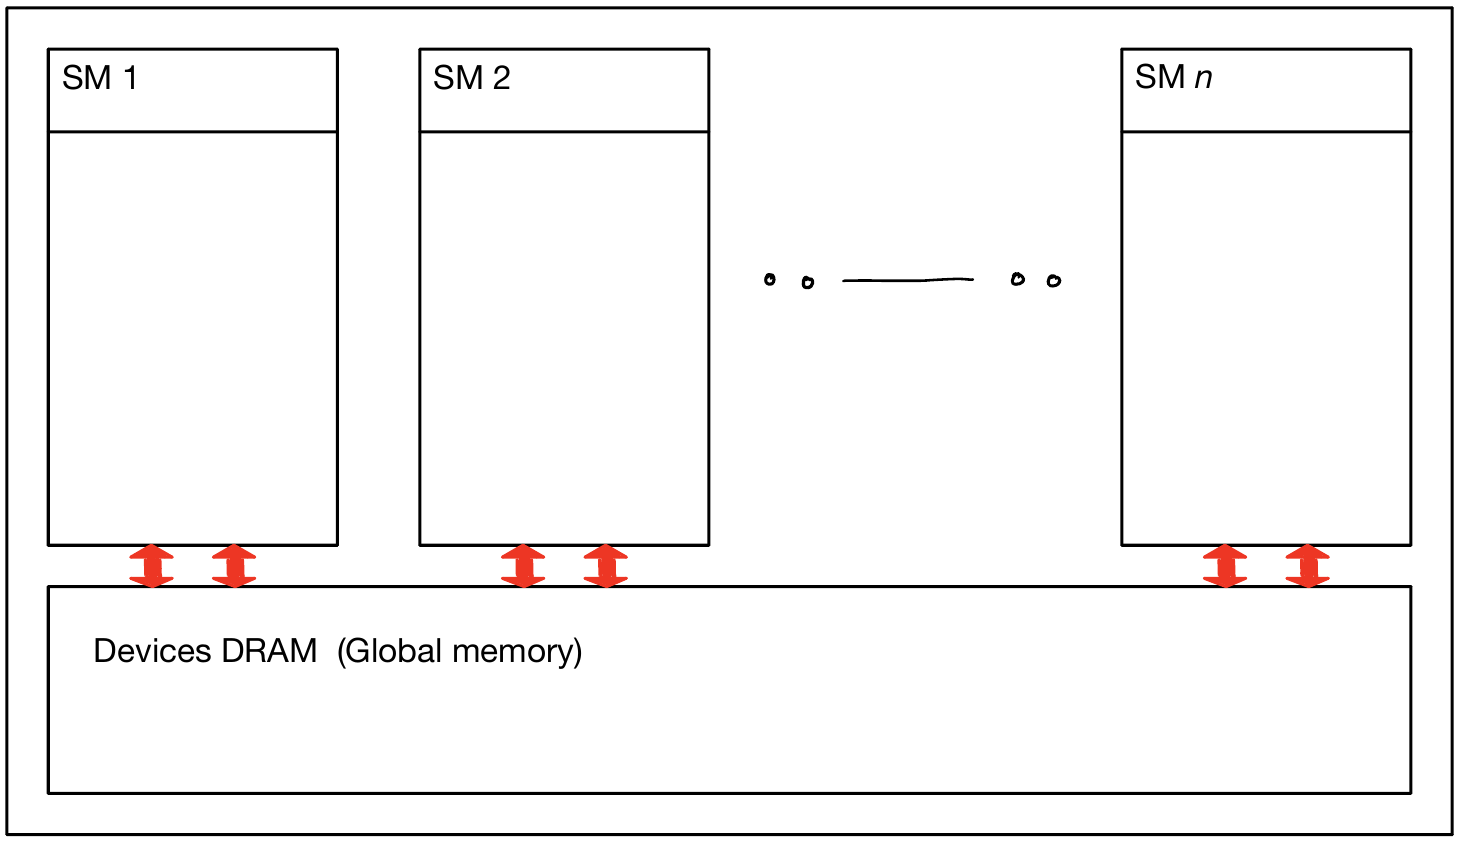
\includegraphics{./assets/GPU_diagram.png}
\caption{GPU Architecture}
\end{figure}


\begin{figure}
\centering
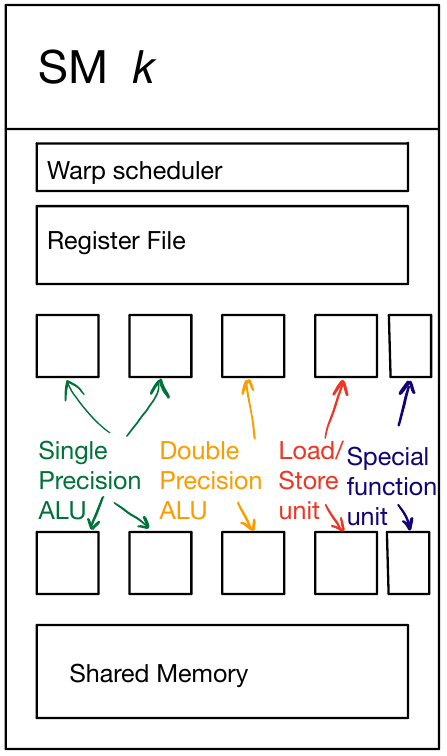
\includegraphics{./assets/SM_diagram.png}
\caption{SM Architecture}
\end{figure}


When a kernel is launched on a GPU we also specify a grid configuration using  the \texttt{blocks} and \texttt{threads} arguments. A grid is composed of "thread blocks" which is a logical collection of threads. The \texttt{blocks} argument defines the block configuration for the grid and the \texttt{threads} argument defines the thread configuration for the thread block.

The GPU schedules each thread block to any available SM with sufficient resources. Blocks can be processed in \textbf{any} order by the GPU. Multiple thread blocks may execute on a single SM if sufficient resources are available. As thread blocks complete execution other thread blocks take their place.

Each thread block contains a \emph{cooperative thread array}(CTA) which is specified by the \texttt{threads} argument. Threads which belong to the same CTA can easily communicate and coordinate with each other because they belong to the same SM. They also have access to a shared memory which is much faster than global memory. The maximum size of a CTA is currently 1024 on NVIDIA hardware.

A small summary of some of the new terms we came across.

\begin{itemize}
\item \emph{thread warp}: A set of threads with a fixed size(32). Instructions in a warp are executed together.


\item \emph{thread block}: A logical collection of threads which can communicate and coordinate easily.


\item \emph{grid}: A logical collection of thread blocks.

\end{itemize}


\end{document}
